\documentclass{article}
\usepackage[utf8]{inputenc}

\title{Sequence to Sequence Learning with Neural Networks}
\author{}
\date{}

\usepackage{natbib}
\usepackage{graphicx}
\usepackage{amsmath}
\usepackage[left=2.5cm,right=2.5cm,top=1cm,bottom=1.25cm]{geometry}
\usepackage{hyperref}
\hypersetup{colorlinks=true,urlcolor=blue}
\pagenumbering{gobble}

\begin{document}

\maketitle

\section*{Link}
\href{https://arxiv.org/abs/1409.3215}{arxiv} 

\section*{Summary}
\begin{itemize}
    \item Deep neural networks require the dimensionality of the inputs and outputs to be known and fixed so they cannot be applied directly to map sequences to sequences. This paper shows a general LSTM structure that can solve sequence to sequence problems. They use one LSTM to to read the input sequence, one timestep at a time t obtain a large fixed dimensional vector representation and use another LSTM to extract output sequence from that vector. To enable the decoder to output arbitrary length sequence they require that each sentence ends with a special end-of-sequence symbol ``EOS".
    \item Using two different LSTMs for encoding and decoding makes it easier to train the LSTM on multiple language pairs simultaneously.
    \item Deep LSTMs significantly outperformed shallow LSTMs for the translation task so they used an LSTM with four layers.
    \item They found it extremely useful to reverse the order of the words in the input sentence(not target sentence). Doing this means that the first few words in the source language were very close to the first few words in the target language. This made optimization by back propagation much easier. This however doesn't change average distance between words in source and target so one might suspect that the translation quality towards the end of the sentences might suffer. However in practice the LSTM trained on reversed source sentences did much better on long sentences than LSTM trained on original ordering. The author didn't mention it explicitly but my guess is when the decoder network starts off in the right track(because it can more easily guess initial words) it becomes easier to make necessary adjustments later down the path. But if it starts with the wrong set of words it becomes much more difficult to get the sentence right because there is no feedback mechanism.
    \item For decoding phase they use beam search which maintains a small number $B$ of partial hypotheses, where a partial hypothesis is a prefix of some translation. At each timestep we extend each partial hypothesis in the beam with every possible word in the vocabulary(the input to decoder at each timestep is the word vector of the last word in the beam). This greatly increases the number of the hypotheses so we discard all but the B most likely hypotheses according to the model’s log probability. As soon as the “EOS” symbol is appended to a hypothesis, it is removed from the beam and is added to the set of complete hypotheses. 
    \item The resulting end to end machine translation system outperforms a phrase-based SMT(Statistical machine translation) baseline on the English to French translation task.
    \item The sentence representations learned by the model are sensitive to word orders while fairly insensitive to replacement of an active voice with a passive voice. This can be seen in \autoref{fig:Figure 1} which is obtained by taking PCA of the final LSTM hidden state generated by the sentences.
    \begin{figure}[t!]
        \centering
        \caption{PCA projection of LSTM hidden states}
        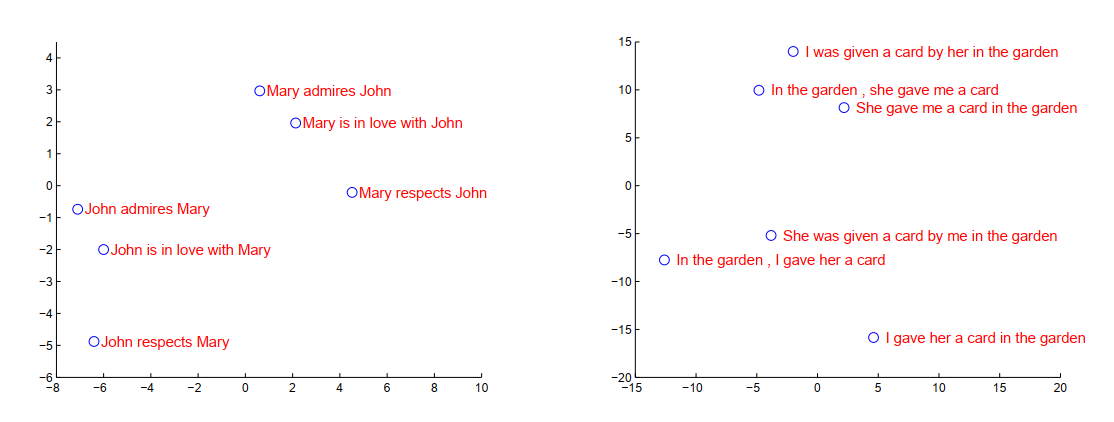
\includegraphics[scale=0.55]{model_analysis.png}
        \label{fig:Figure 1}
    \end{figure}
    \item There was no degradation in performance on sentences with less than 35 words which shows that LSTM can recover long term dependency. There is minor degradation on the longest sentences(~70 word long)
\end{itemize}

\end{document}
